\documentclass{standalone}
\usepackage{tikz}
\usetikzlibrary{patterns, positioning}
\usepackage[sfdefault]{ClearSans} %% option 'sfdefault' activates Clear Sans as the default text font
\usepackage[T1]{fontenc}

\begin{document}
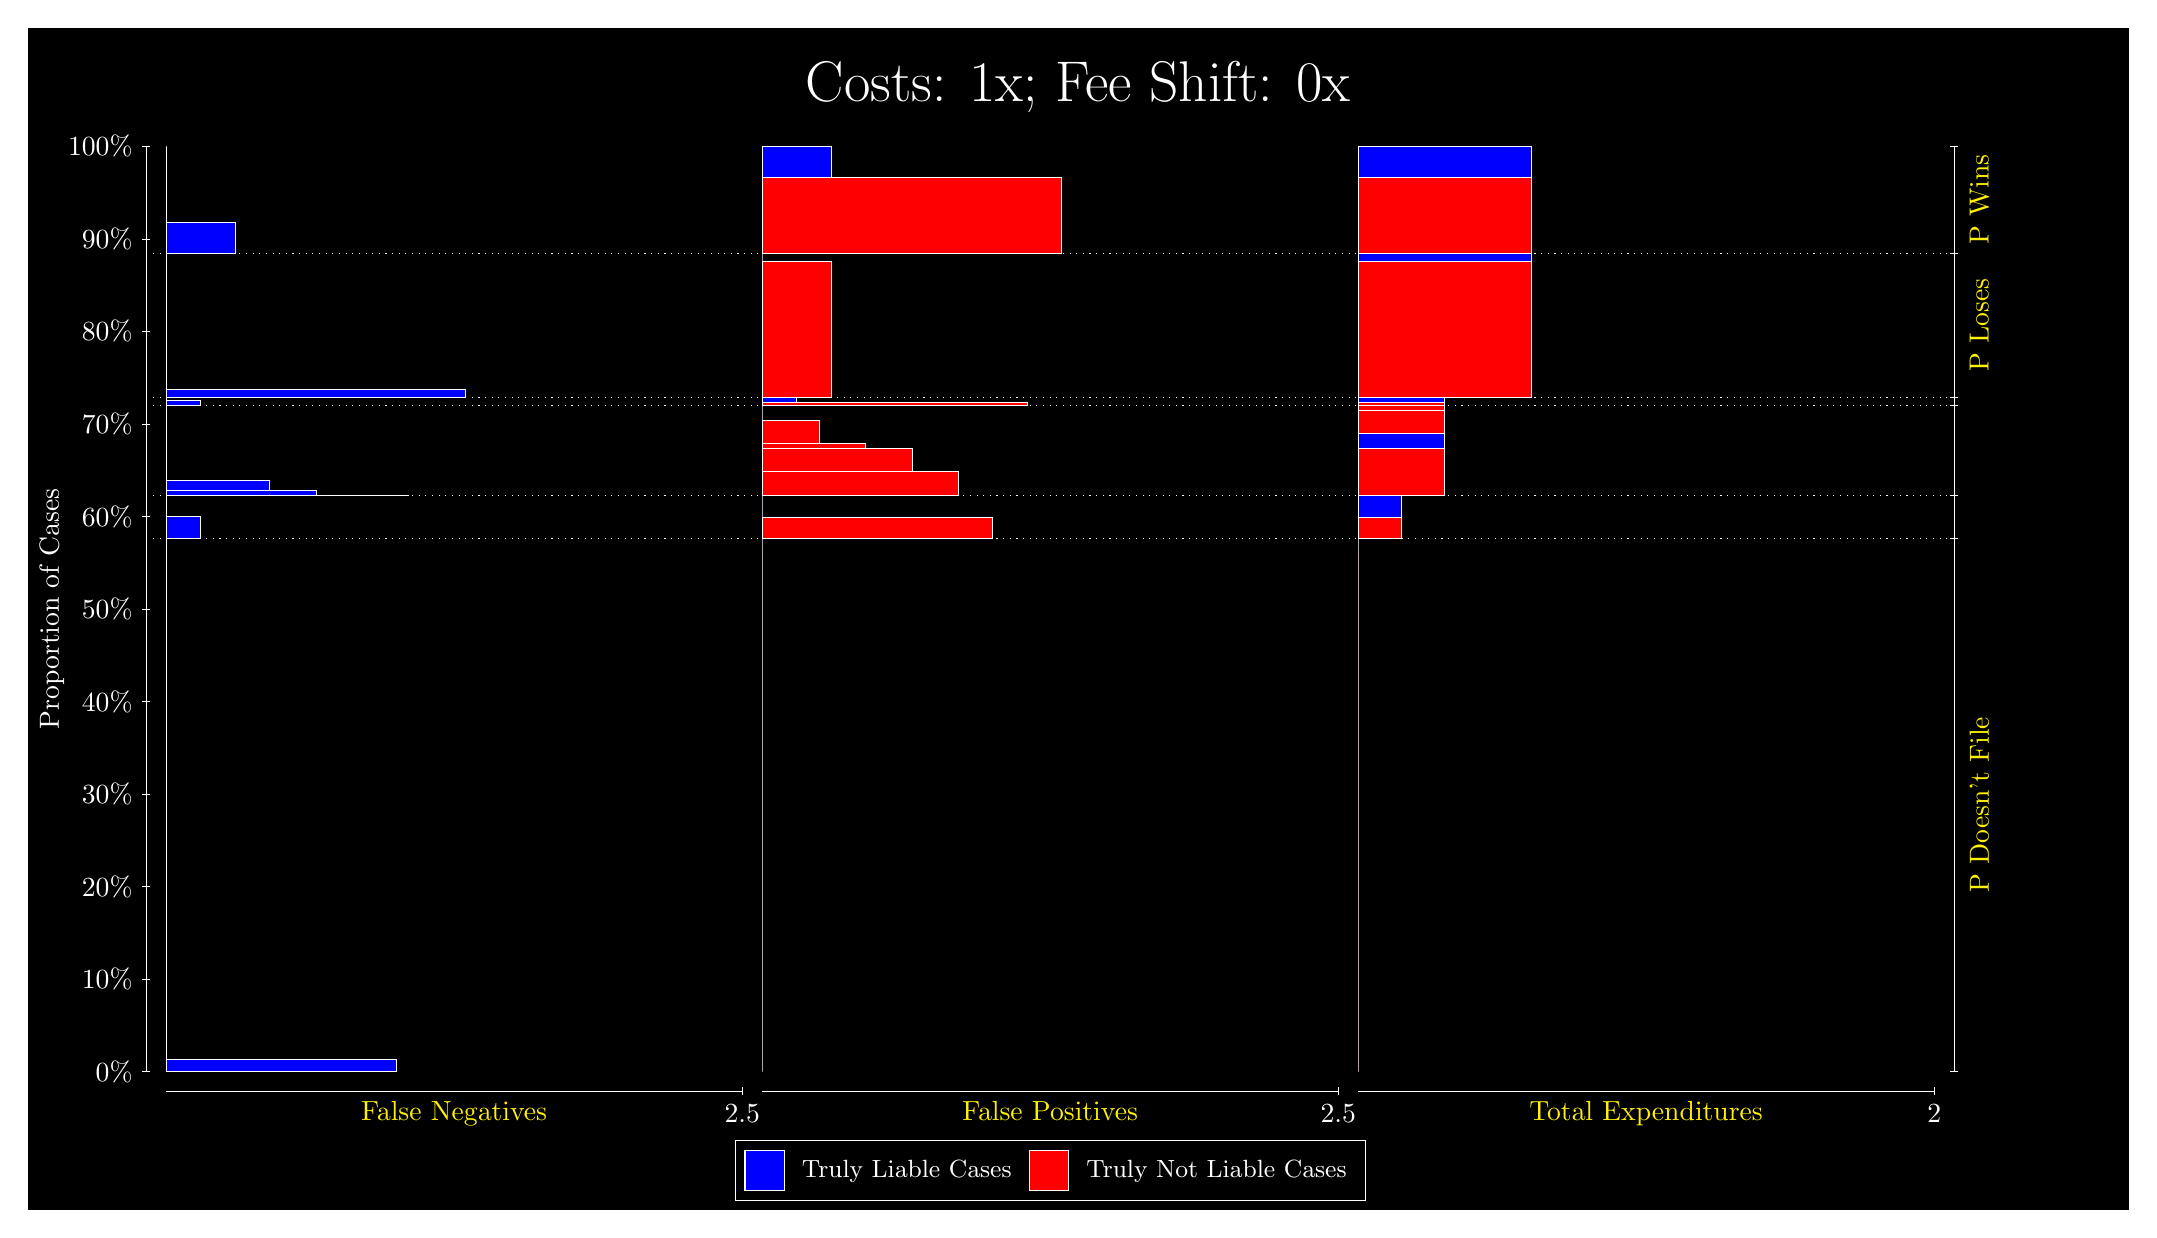
\begin{tikzpicture}
\draw[fill=black] (0,0) rectangle (26.667,15);
\draw[text=white] (0,13.5) rectangle (26.667,15) node[midway] {\huge Costs: 1x; Fee Shift: 0x};
\draw[white, very thin] (1.5,1.75) -- (1.5,13.5);
\node[rotate=90, text=white, anchor=center] at (0.3, 7.625) {Proportion of Cases};
\draw[white, very thin] (1.45,1.75) -- (1.55,1.75);
\node[text=white, anchor=east] at (1.45, 1.75) {0\%};
\draw[white, very thin] (1.45,2.925) -- (1.55,2.925);
\node[text=white, anchor=east] at (1.45, 2.925) {10\%};
\draw[white, very thin] (1.45,4.1) -- (1.55,4.1);
\node[text=white, anchor=east] at (1.45, 4.1) {20\%};
\draw[white, very thin] (1.45,5.275) -- (1.55,5.275);
\node[text=white, anchor=east] at (1.45, 5.275) {30\%};
\draw[white, very thin] (1.45,6.45) -- (1.55,6.45);
\node[text=white, anchor=east] at (1.45, 6.45) {40\%};
\draw[white, very thin] (1.45,7.625) -- (1.55,7.625);
\node[text=white, anchor=east] at (1.45, 7.625) {50\%};
\draw[white, very thin] (1.45,8.8) -- (1.55,8.8);
\node[text=white, anchor=east] at (1.45, 8.8) {60\%};
\draw[white, very thin] (1.45,9.975) -- (1.55,9.975);
\node[text=white, anchor=east] at (1.45, 9.975) {70\%};
\draw[white, very thin] (1.45,11.15) -- (1.55,11.15);
\node[text=white, anchor=east] at (1.45, 11.15) {80\%};
\draw[white, very thin] (1.45,12.325) -- (1.55,12.325);
\node[text=white, anchor=east] at (1.45, 12.325) {90\%};
\draw[white, very thin] (1.45,13.5) -- (1.55,13.5);
\node[text=white, anchor=east] at (1.45, 13.5) {100\%};

\draw[white, very thin] (24.457,1.75) -- (24.457,13.5);
\draw[white, very thin] (24.407,1.75) -- (24.507,1.75);
\node[anchor=west] at (24.407, 1.75) {};
\draw[white, very thin] (24.407,8.5226) -- (24.507,8.5226);
\node[anchor=west] at (24.407, 8.5226) {};
\draw[white, very thin] (24.407,9.0628) -- (24.507,9.0628);
\node[anchor=west] at (24.407, 9.0628) {};
\draw[white, very thin] (24.407,10.213) -- (24.507,10.213);
\node[anchor=west] at (24.407, 10.213) {};
\draw[white, very thin] (24.407,10.311) -- (24.507,10.311);
\node[anchor=west] at (24.407, 10.311) {};
\draw[white, very thin] (24.407,12.144) -- (24.507,12.144);
\node[anchor=west] at (24.407, 12.144) {};
\draw[white, very thin] (24.407,13.5) -- (24.507,13.5);
\node[anchor=west] at (24.407, 13.5) {};

\draw[white, very thin, fill=blue] (1.75,1.75) rectangle (4.6775,1.8994);
\draw[white, very thin, fill=red] (1.75,1.8994) rectangle (1.75,8.5226);
\draw[white, very thin, fill=blue] (1.75,8.5226) rectangle (2.1891,8.8005);
\draw[white, very thin, fill=red] (1.75,8.8005) rectangle (1.75,9.0628);
\draw[white, very thin, fill=blue] (1.75,9.0628) rectangle (4.8239,9.069);
\draw[white, very thin, fill=blue] (1.75,9.069) rectangle (4.2384,9.0734);
\draw[white, very thin, fill=blue] (1.75,9.0734) rectangle (3.6529,9.1274);
\draw[white, very thin, fill=blue] (1.75,9.1274) rectangle (3.0674,9.2586);
\draw[white, very thin, fill=red] (1.75,9.2586) rectangle (1.75,10.213);
\draw[white, very thin, fill=blue] (1.75,10.213) rectangle (2.1891,10.272);
\draw[white, very thin, fill=red] (1.75,10.272) rectangle (1.75,10.311);
\draw[white, very thin, fill=blue] (1.75,10.311) rectangle (5.5558,10.418);
\draw[white, very thin, fill=red] (1.75,10.418) rectangle (1.75,12.144);
\draw[white, very thin, fill=blue] (1.75,12.144) rectangle (2.6283,12.531);
\draw[white, very thin, fill=red] (1.75,12.531) rectangle (1.75,13.5);
\draw[white, very thin, fill=red] (9.3189,1.75) rectangle (9.3189,8.3733);
\draw[white, very thin, fill=blue] (9.3189,8.3733) rectangle (9.3189,8.5226);
\draw[white, very thin, fill=red] (9.3189,8.5226) rectangle (12.246,8.785);
\draw[white, very thin, fill=blue] (9.3189,8.785) rectangle (9.3189,9.0628);
\draw[white, very thin, fill=red] (9.3189,9.0628) rectangle (11.807,9.3669);
\draw[white, very thin, fill=red] (9.3189,9.3669) rectangle (11.222,9.6689);
\draw[white, very thin, fill=red] (9.3189,9.6689) rectangle (10.636,9.7282);
\draw[white, very thin, fill=red] (9.3189,9.7282) rectangle (10.051,10.018);
\draw[white, very thin, fill=blue] (9.3189,10.018) rectangle (9.3189,10.213);
\draw[white, very thin, fill=red] (9.3189,10.213) rectangle (12.686,10.253);
\draw[white, very thin, fill=blue] (9.3189,10.253) rectangle (9.758,10.311);
\draw[white, very thin, fill=red] (9.3189,10.311) rectangle (10.197,12.037);
\draw[white, very thin, fill=blue] (9.3189,12.037) rectangle (9.3189,12.144);
\draw[white, very thin, fill=red] (9.3189,12.144) rectangle (13.125,13.113);
\draw[white, very thin, fill=blue] (9.3189,13.113) rectangle (10.197,13.5);
\draw[white, very thin, fill=red] (16.888,1.75) rectangle (16.888,8.3733);
\draw[white, very thin, fill=blue] (16.888,8.3733) rectangle (16.888,8.5226);
\draw[white, very thin, fill=red] (16.888,8.5226) rectangle (17.437,8.785);
\draw[white, very thin, fill=blue] (16.888,8.785) rectangle (17.437,9.0628);
\draw[white, very thin, fill=red] (16.888,9.0628) rectangle (17.986,9.6689);
\draw[white, very thin, fill=blue] (16.888,9.6689) rectangle (17.986,9.8542);
\draw[white, very thin, fill=red] (16.888,9.8542) rectangle (17.986,10.144);
\draw[white, very thin, fill=blue] (16.888,10.144) rectangle (17.986,10.15);
\draw[white, very thin, fill=red] (16.888,10.15) rectangle (17.986,10.209);
\draw[white, very thin, fill=blue] (16.888,10.209) rectangle (17.986,10.213);
\draw[white, very thin, fill=red] (16.888,10.213) rectangle (17.986,10.253);
\draw[white, very thin, fill=blue] (16.888,10.253) rectangle (17.986,10.311);
\draw[white, very thin, fill=red] (16.888,10.311) rectangle (19.083,12.037);
\draw[white, very thin, fill=blue] (16.888,12.037) rectangle (19.083,12.144);
\draw[white, very thin, fill=red] (16.888,12.144) rectangle (19.083,13.113);
\draw[white, very thin, fill=blue] (16.888,13.113) rectangle (19.083,13.5);
\draw[white, dotted] (1.5,8.5226) -- (24.457,8.5226);
\draw[white, dotted] (1.5,9.0628) -- (24.457,9.0628);
\draw[white, dotted] (1.5,10.213) -- (24.457,10.213);
\draw[white, dotted] (1.5,10.311) -- (24.457,10.311);
\draw[white, dotted] (1.5,12.144) -- (24.457,12.144);
\draw[white, very thin] (1.75,1.5) -- (9.0689,1.5);
\node[text=yellow, anchor=north] at (5.4094, 1.5) {False Negatives};
\draw[white, very thin] (9.0689,1.45) -- (9.0689,1.55);
\node[text=white, anchor=north] at (9.0689, 1.45) {2.5};

\draw[white, very thin] (9.3189,1.5) -- (16.638,1.5);
\node[text=yellow, anchor=north] at (12.978, 1.5) {False Positives};
\draw[white, very thin] (16.638,1.45) -- (16.638,1.55);
\node[text=white, anchor=north] at (16.638, 1.45) {2.5};

\draw[white, very thin] (16.888,1.5) -- (24.207,1.5);
\node[text=yellow, anchor=north] at (20.547, 1.5) {Total Expenditures};
\draw[white, very thin] (24.207,1.45) -- (24.207,1.55);
\node[text=white, anchor=north] at (24.207, 1.45) {2};

\node[text=yellow, centered, rotate=90] at (24.777, 5.1363) {P Doesn't File};



\node[text=yellow, centered, rotate=90] at (24.777, 11.228) {P Loses};
\node[text=yellow, centered, rotate=90] at (24.777, 12.822) {P Wins};

\draw (12.978300999999998,1.5) node[draw=none] (baseCoordinate) {};
\begin{scope}[align=center]
        \matrix[scale=0.5, draw=white, below=0.5cm of baseCoordinate, nodes={draw}, column sep=0.1cm]{
            \node[rectangle, draw, minimum width=0.5cm, minimum height=0.5cm, fill=blue] {}; &
            \node[draw=none, font=\small, text=white] (B) {Truly Liable Cases}; &
            \node[rectangle, draw, minimum width=0.5cm, minimum height=0.5cm, fill=red] {}; &
            \node[draw=none, font=\small, text=white] (B) {Truly Not Liable Cases}; \\
            };
\end{scope}

\end{tikzpicture}
\end{document}